\subsection{La estructura de los papers científicos}

Si bien los distintos congresos, jornadas, libros o publicaciones, mantienen un cierto grado de independencia con respecto a los formatos y contenidos de los trabajos que publican, es importante mencionar que la producción científica se apega a algunas normas, ya sea formales o de hecho, que facilitan la distribución y análisis del contenido generado.

Los procesos de producción científica dan lugar generalmente a documentos que, si bien no son idénticos en el formato, tienen un grado de coherencia muy importante para posibilitar el análisis y entendimiento por parte de otros investigadores, distintos a los que generaron el contenido.

Muchos documentos siguen el formato conocido como IMRyD (por la sigla de Introducción, Métodos, Resultados y Discusión \cite{del2007difusion}, ver Figura \ref{fig:imryd}) ya sea literalmente o como una guía a la hora de estructurar los documentos.

\begin{figure}[H]
	\centering
	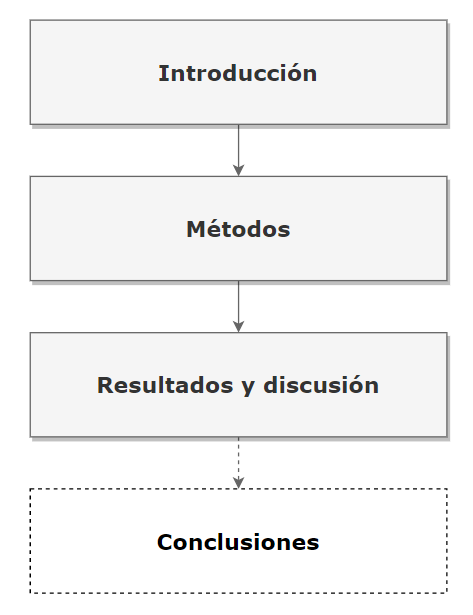
\includegraphics[width=0.6\linewidth]{images/imryd}
	\caption{\textbf{Secciones del modelo IMRyD}}
	\label{fig:imryd}
\end{figure}

Esta guía, en cuanto al formato, le da a los artículos resultantes un orden lógico, los hace comparables unos con otros, estructura el contenido, secuencia la lectura de los resultados y provee una forma simple y útil para ayudar a los autores a producir artículos que pueden ser correctamente analizados, evaluados por sus pares, editados y publicados.

La secciones del formato IMRyD son las siguientes:

\begin{description}
	\item[Introducción:] Busca responder a la motivación de la elaboración del documento y al objeto de estudio del mismo. A modo de resumen, se puede decir que la introducción responde a las preguntas ``¿Qué se investigó?'', ``¿Por qué se investigó?''.
	\item[Métodos:] En la sección de métodos (a veces denominada Métodos y Materiales) se elaboran todas las técnicas utilizadas para realizar las experiencias de investigación, los elementos utilizados, los datos sobre los que se trabajó, las referencias consultadas, etc. Busca responder a la pregunta ``¿Cómo se realizó la investigación?''
	\item[Resultados:] En la sección de Resultados se exponen todos los producidos por la tarea de investigación. Los resultados pueden tomar diversas formas, tales como tablas de datos, algoritmos, fórmulas matemáticas, etc. Esta sección busca responder a la pregunta ``¿Qué se encontró durante la investigación?'' pero teniendo especial cuidado de no realizar interpretaciones sobre dichos resultados.
	\item[Discusión:] La última sección recomendada por el formato IMRyD es la sección de Discusión de los resultados. Esta sección es quizá la más importante de todo el trabajo de investigación ya que pone en contexto la importancia de los resultados obtenidos. En la discusión se plantean las hipótesis que se pueden haber confirmado o refutado por los resultados, las relaciones entre los resultados y otros estudios, de otros autores, en la misma vía o complementarios, así como las implicancias de los resultados encontrados dentro del cúmulo de conocimientos del área bajo estudio.
\end{description}

Si bien las mencionadas anteriormente son las secciones formalmente reconocidas por el formato IMRyD, en muchos casos se incluye una sección de Conclusiones que resume los puntos más importantes de los Resultados y la Discusión del artículo.

\subsection{Los datos básicos extraíbles}

A la hora de plantear una base de datos cienciométrica es crucial analizar la fuente primaria de los datos que se deberán procesar. Esta fuente primaria no es otra que los datos provistos por los documentos publicados en actas, journals, libros, etc.

En tal sentido, la estandarización del formato y la estructura de dichos documentos cobra una gran importancia.

A continuación se explorarán las distintas secciones que componen un documento científico y se analizará la información que se puede extraer de cada uno de ellos.

\subsubsection{Título}

El título del documento expresa de forma resumida y concisa el contenido del trabajo de investigación. Del análisis del título del artículo se pueden obtener los conceptos principales que formarán parte del artículo de investigación.

\subsubsection{Abstract o resumen}

En el resumen del artículo se encuentra una explicación breve del contenido general del trabajo. El análisis de esta sección permitiría establecer los conceptos generales vertidos en el resto del artículo, las relaciones entre los mismos, la determinación del tipo de trabajo (experimental, exploratorio, comparativo, etc.) así como algunos de los resultados más importantes.

\subsubsection{Autores y filiación}

Todo artículo científico debe incluir información de su autor o autores, así como de la filiación de los mismos con las organizaciones en donde desarrollan sus actividades. La información de los datos personales de los autores, su información de contacto y los datos de organizaciones o universidades, brindan información valiosa sobre producción científica, tanto sea desde el punto de vista de la producción personal de los autores como de la producción científica de las organizaciones donde los mismos se desempeñan.

\subsubsection{Cuerpo del artículo}

La mayor parte del texto está presente en el cuerpo del artículo, el cual puede contener secciones y subsecciones de acuerdo a las necesidades de organización del autor y a los criterios impuestos por la publicación o congreso al cual se va a enviar el texto.

En el cuerpo del artículo se encuentran los planteos introductorios, los métodos y los recursos utilizados para la investigación, la exposición de resultados y el análisis de los mismos así como los pasos futuros que se prevén para la investigación.

\subsubsection{Referencias}

En la sección de referencias, ubicada al final del artículo o paper científico, se encuentran los datos de otras obras y autores consultados para el desarrollo del trabajo. Si bien el formato específico en el cual se registran las referencias puede variar de acuerdo al formato del trabajo, lo cierto es que los tipos de referencias bibliográficas están estandarizadas en un conjunto acotado, que define tanto el formato textual que deben tener las citas, como la manera de referenciar ciertos datos concretos como ser el nombre de la publicación, el año, los autores, el tipo de referencia, etc.

\subsection{Relaciones con bases de datos externas}

Una de las principales ventajas que proveen las redes de información globales es el acceso a grandes fuentes de información a un coste extremadamente bajo. Desde su misma concepción la World Wide Web tuvo como finalidad principal la posibilidad de compartir documentos de investigación en el entorno de CERN (de la sigla en francés de Conseil Européen pour la Recherche Nucléaire, Consejo Europeo para la Investigación Nuclear), donde fue concebida por Tim Berners-Lee \cite{segal1995short}, creciendo a partir de ese punto para englobar otras actividades y participantes.

Hoy en día existen enormes bases de datos y repositorios de documentación científica, ya sean comerciales \cite{bakkalbasi2006three} o de acceso abierto \cite{minniti2018mapping}, con diferentes funcionalidades y capacidades de consulta (un listado de los principales se puede encontrar en la Tabla \ref{tab:repositorios}).

Por tal motivo ningún sistema de información cienciométrica puede estar completo sin contar, en alguna medida, con la capacidad de conectarse a esos repositorios y enlazar la propia información a la que radica en bases de datos externas \cite{garfield2006citation}.

\begin{table}[ht]
	\centering	
	\caption{\textbf{Algunos repositorios que incluyen indexación de citas}}
	\begin{tabularx}{.8\linewidth}{Xc}
		\toprule
		\textbf{Repositorio}&\textbf{Tipo}\\
		\midrule
		Open Citation Index&Abierto\\
		Google Scholar Index&Abierto\\
		Web of Science&Pago\\
		Scopus&Pago\\
		SciELO&Abierto\\
		\bottomrule
	\end{tabularx}
	
	\label{tab:repositorios}
\end{table}%

Quizá una de las funcionalidades más útiles a la hora de diseñar esa interacción sea la del referenciamiento de citas, que brinda información sobre las citas existentes entre distintos autores y trabajos de investigación y permite acceder al material que se utilizó para la elaboración de dicho trabajo \cite{harzing2008google,bakkalbasi2006three}.

Estas bases de datos externas a menudo ofrecen interfaces y API's de acceso (por suscripción, en el caso de los repositorios comerciales) que permiten que un software de terceros pueda consultar y/o validar información de referencias de una manera sencilla y rápida.

\subsection{Algunos análisis cienciométricos relevantes}

El desarrollo de una base de datos cienciométrica no reduce su utilidad al mero almacenamiento de la información sino que busca ser un repositorio de información para realizar análisis tanto descriptivos como prospectivos, que tengan como finalidad:

\begin{itemize}
	\item El descubrimiento de relaciones no evidentes entre investigadores, instituciones, ámbitos científicos, etc.
	\item El trazado de redes de colaboración que potencien la labor de investigadores y centros de investigación.
	\item El análisis de líneas de investigación actuales y futuras como un sistema de ayuda para nuevos investigadores que se estén iniciando.
	\item La detección de grupos aislados que puedan beneficiarse de la interacción con otros grupos de la red de relaciones.
	\item La sugerencia, a los investigadores, de temáticas complementarias que puedan dar una perspectiva más amplia a sus trabajos.
	\item La información, a las instituciones, de un mapa de las líneas en que trabajan sus investigadores, comparativo con los de otras instituciones, en vistas a acuerdos de colaboración e intercambio de experiencias.
	\item El análisis temporal de la investigación científica para detectar temáticas en decadencia o en auge, para direccionar mejor las políticas de ciencia y tecnología de instituciones educativas y otras organizaciones.
	\item Estudiar la dispersión y la obsolescencia de la literatura científica.
	\item Analizar la productividad de editores, autores, organizaciones, países, etc. en lo que a producción científica se refiere.
\end{itemize}

Es importante mencionar que muchos de los análisis e indicadores mencionados \cite{spinak1998indicadores} en el listado precedente tienen una correlación directa con las políticas públicas de promoción y fortalecimiento de la infraestructura científica y tecnológica de un país \cite{de1999science}, y en última instancia con los desarrollos productos de esas políticas, impactando en última instancia en la calidad de vida de la población \cite{miguel2008aproximacion}.

\subsubsection{El flujo de trabajo del análisis cienciométrico}

Existen ciertas etapas dentro de la elaboración de un análisis cienciométrico (ver Figura \ref{fig:flow}), que si bien no están estandarizadas, son lo suficientemente comunes y extendidas como para considerarse un marco de trabajo válido \cite{cardona2017analisis}. En todas ellas tiene, en alguna medida, intervención una base de datos de información cienciométrica.

\begin{figure*}[!h]
	\centering
	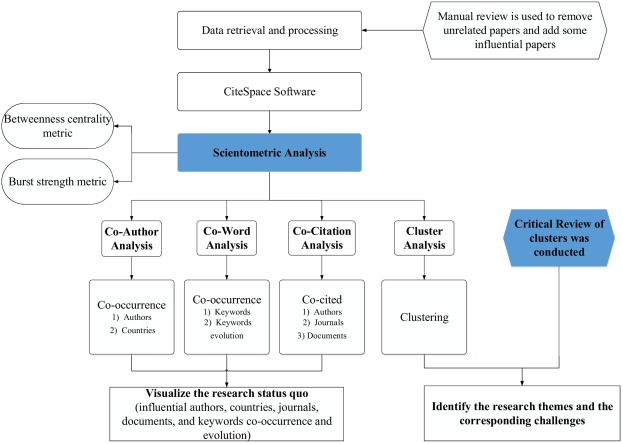
\includegraphics[width=0.65\linewidth]{images/flow}
	\caption{\textbf{Flujo de trabajo del análisis cienciométrico}}
	\label{fig:flow}
\end{figure*}

Todo esfuerzo de análisis cienciométrico comienza mediante la recopilación de la documentación sobre la que se va a trabajar. Dicho relevamiento puede tomar la forma de actividades manuales o ser un proceso automatizado, por medio de la lectura o descarga de los documentos, la detección de sus atributos característicos y el almacenamiento de los mismos en el repositorio cienciométrico.

\paragraph{El análisis de citas}
Una vez cargados los datos en el almacenamiento se procede al primer análisis netamente cienciométrico, el análisis de citas. Dicho análisis implica la búsqueda de información relacionada a cada uno de los documentos bajo tratamiento, de manera de identificar los trabajos citados, y los autores de los mismos. Esto lleva a la creación de una lista de citas, que contiene el nombre de la obra citada, los datos de los autores e información sobre la publicación en dónde se encuentran, la fecha de publicación, etc.

Este primer análisis comienza a dar forma a la red de relaciones que unen, en esta etapa, documentos, autores y publicaciones.

En una segunda etapa se realizan análisis cienciométricos más detallados que pueden realizarse de manera simultánea o secuencial, de acuerdo a las necesidades.

\paragraph{El análisis de co-autorías}
El análisis de co-autoría busca determinar las relaciones entre distintos autores del mismo trabajo, y es utilizado para determinar las redes de colaboración, compuesta por aquellas personas que colaboran entre sí para dar lugar a la publicación de un artículo determinado. 

No se debe confundir la colaboración directa, como la mencionada en este punto, con la cita, que si bien implica el trabajo en temáticas afines, no indica una colaboración directa entre los autores.

\paragraph{Ocurrencia de palabras clave}
En otro paso del proceso de análisis se realiza un análisis de ocurrencia de palabras clave. En este análisis se busca establecer relaciones entre artículos que tratan la misma temática, ya sea de manera total o parcial, de acuerdo a la cantidad de coincidencias. 

Este análisis es particularmente importante ya que determina un conjunto de documentos asociados a una temática determinada, sin tener en cuenta que los autores puedan o no ser comunes. Establece, por así decirlo, el conjunto de conocimiento disponible sobre una temática particular.

\paragraph{El análisis de co-cita}
El análisis de co-cita es un procedimiento mediante el cual se detectan referencias recíprocas entre artículos de autores. Este modelo es muy común entre autores que no trabajan directamente en grupo pero cuyos intereses son similares y cada uno utiliza como referencias los trabajos del otro \cite{wei2020document}. Es un patrón muy interesante para determinar posibilidades de colaboración directa a partir de referencias indirectas.

\paragraph{Clustering}
En el análisis de clustering \cite{liu2018co} se toman trabajos de áreas científicas enteras y los mismos se agrupan de acuerdo a las palabras clave o a contenidos dentro del texto del documento. Si bien guarda algunas similitudes con el análisis de palabras clave, el clustering busca generalizar y abarcar un nivel superior, hacia áreas completas de conocimiento.

Esto es posible mediante la utilización de ciertos diccionarios, formales o no, que mapean palabras clave a ámbitos de conocimiento estandarizados y nomenclados.

Es importante mencionar que distintas técnicas de clustering pueden llevar a agrupaciones diferentes de acuerdo a los criterios aplicados, por lo que no es infrecuente la revisión de los resultados de forma manual o semi automática, para evitar categorizaciones erróneas que puedan llevar a sacar conclusiones equivocadas.

\subsubsection{Importancia de los distintos tipos de análisis}

Existen dos tipos principales de utilidad en los diversos tipos de análisis cienciométricos, el conocimiento del estado de la ciencia y los estudios prospectivos sobre la misma.

Los análisis de co-ocurrencia, co-autoría, palabras clave y co-cita, lo que buscan es determinar el mapa actual del conocimiento, los temas sobre los que se está trabajando, los autores que están investigando y las temáticas involucradas.

Pero cuando se recurre a los análisis de cluster, sobre todo si se conjuga con la evolución temporal de las distintas disciplinas, se cuenta con una importante herramienta prospectiva que permite analizar no sólo la historia de la investigación en cada campo sino también realizar estimaciones de la dirección en la que se está moviendo la investigación sobre un tema o una rama del conocimiento.

Este análisis permite determinar no sólo qué líneas de investigación están decayendo sino cuáles están surgiendo, en qué direcciones, sobre qué ámbitos es esperable que existan avances y en qué autores está recayendo la atención debido a sus aportes. La capacidad de poder estimar el movimiento futuro de los avances científicos es una herramienta de un enorme valor para la planificación de políticas de ciencia y tecnología eficaces, ya sea en el ámbito público o privado, educativo, político o productivo.

\subsection{El diseño de la base de datos cienciométrica}

A fin de posibilitar la obtención de los indicadores y análisis cienciométricos mencionados en el punto anterior, es imprescindible la implementación de una base de datos de información cienciométrica para la cual se deben tener en cuenta un conjunto de criterios que permitan obtener información de calidad, relevante y actualizada, adecuada para realizar los análisis necesarios.

Una base de datos cienciométrica es un sistema de representación del conocimiento, específicamente de aquel asociado a la producción científica.

Actualmente se deben tener en cuenta al menos cuatro criterios fundamentales a la hora de diseñar un sistema de representación del conocimiento en cualquier dominio dado \cite{van2008handbook}:

\begin{description}
	\item [Adecuación Representacional:] Habilidad para representar todas las clases de conocimiento que son necesarias en el dominio.
	\item [Adecuación Inferencial:] Habilidad de manipular estructuras de representación de tal manera que devengan o generen nuevas estructuras que correspondan a nuevos conocimientos inferidos de los anteriores.
	\item [Eficiencia Inferencial:] Capacidad del sistema para incorporar información adicional a la estructura de representación, llamada metaconocimiento, que puede emplearse para focalizar la atención de los mecanismos de inferencia con el fin de optimizar los cómputos.
	\item [Eficiencia en la Adquisición:] Capacidad de incorporar fácilmente nueva información. Idealmente el sistema por sí mismo deberá ser capaz de controlar la adquisición de nueva información y su posterior representación.
\end{description}

Estos criterios son los que se deben tener en cuenta a la hora de analizar las distintas alternativas disponibles para diseñar una base de datos cienciométrica.

Al momento de diseñar tal base de datos dos cuestiones principales son las que deben resolverse:

\begin{enumerate}
	\item ¿Cuál es el uso principal que se le va a dar a la base de datos?
	\item ¿Cuál es el modelo más apropiado para la representación de la información?
\end{enumerate}

Ambos elementos no son completamente independiente sino que, por el contrario, se complementan e influyen mutuamente, a tal punto que en el diseño se tienen que combinar ambos y no son infrecuentes los casos en los cuales existe un proceso, iterativo e incremental, que va refinando progresivamente ambos elementos a medida que se va avanzando en el proceso y se logra un conocimiento cada vez mayor del dominio en cuestión.

A la primera pregunta se la debe enfocar desde el punto de vista de los usuarios finales, para lo cual hay que definirlos, ya que serán ellos los que utilicen la información.

En la gran mayoría de los casos existen dos tipos de usuarios representativos de las bases de datos cienciométricas:

\begin{description}
	\item[Usuarios de consulta:] Estos usuarios realizan consultas puntuales a la base de datos, generalmente buscando información sobre autores, artículos o líneas de investigación puntuales. Generalmente tienen criterios de búsqueda bastante bien definidos y requieren un conjunto de resultados de pequeño tamaño.
	\item[Usuarios analíticos] Este perfil de usuarios realiza operaciones más masivas sobre la base de datos, en la búsqueda de encontrar información analítica y de indicadores generales. Generalmente los criterios de búsqueda no son demasiado exactos, debido al carácter exploratorio de las tareas que desarrolla, y por lo tanto las consultas más genéricas obtienen resultados más amplios, lo que se traduce en una mayor cantidad de registros.
\end{description}

Para afrontar la cuestión de cuál es el modelo más apropiado para la representación de la información se debe tener en cuenta la natural heterogeneidad de los datos que se pueden extraer de los artículos científicos. 

Si bien el formato y estructura de dichos documentos está en gran medida estandarizada, también es real que las relaciones entre las entidades que componen un trabajo de investigación pueden ser muy variables y variadas. Y es precisamente en el marco de estas relaciones donde radica el mayor valor del análisis cienciométrico.

Algunas de las posibles relaciones que se pueden establecer entre las entidades de un modelo de información cienciométrica se encuentran en la Tabla \ref{tab:relaciones}.

\begin{table}[ht]
	\centering	
	\caption{\textbf{Relaciones entre entidades cienciométricas}}
	\begin{tabularx}{0.9\linewidth}{rcccc}
		\toprule
		&Autor&Artículo&Tema&Institución\\
		\midrule
		Autor&{\tiny colabora con}&{\tiny publica}&{\tiny investiga}&{\tiny pertenece a}\\
		Artículo&{\tiny publicado por}&{\tiny referencia}&{\tiny pertenece a}& {\tiny avalado por}\\
		Tema&{\tiny investigado por}&{\tiny incluye}& {\tiny relacionado con} & {\tiny investigado por} \\
		Institución& {\tiny avala} & {\tiny avala} & {\tiny investiga} & {\tiny colabora}\\
		\bottomrule
	\end{tabularx}
	
	
	\label{tab:relaciones}
\end{table}%

Si consideramos la tabla mencionada podemos ver que existen multitud de relaciones N-N (relaciones de todos con todos) lo que puede llevar rápidamente a un crecimiento exponencial de la cantidad de relaciones que un modelo de datos debe manejar.

Si bien en la actualidad el modelo de datos relacional es un modelo probado, conocido y estable, no es el más recomendable en este escenario debido al aumento exponencial de los tiempos de búsqueda al contar con multitud de relaciones de tipo N-N \cite{kunii1987dbms}. 

Desde hace un tiempo y con el advenimiento de disciplinas como el Data Minning, el Data Warehousing y algunas aplicaciones de Inteligencia Artificial y Machine Learning, se están impulsando modelos alternativos que no sufran las limitaciones del modelo relacional y que permitan gestionar eficientemente grandes cantidades de datos heterogéneos \cite{vicknair2010comparison}. 

El equipo de investigación ha realizado con anterioridad experiencias con la utilización de bases de datos de grafos y las mismas se consideran, hasta el momento, una de las alternativas más prometedoras.

\subsubsection{Definición de grafo}

En matemáticas y en ciencias de la computación se define a un grafo como un	conjunto de objetos denominados vértices (también pueden mencionarse como nodos), relacionados por enlaces llamados aristas o arcos (ver Figura \ref{fig:grafo}). Estas relaciones establecen una asociación binaria entre dos nodos, la cual puede ser dirigida, en uno u otro sentido, o no.

\begin{figure}
	\centering
	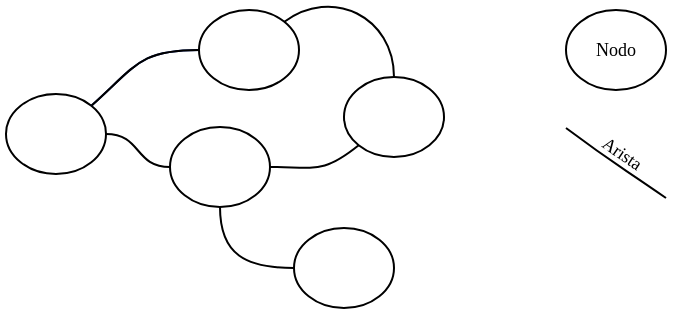
\includegraphics[width=0.7\linewidth]{images/grafo}
	\caption{\textbf{Ejemplo de grafo no dirigido}}
	\label{fig:grafo}
\end{figure}

Los grafos pueden tener información asociada tanto a los nodos como a los arcos, denominándose en este caso grafos etiquetados \cite{van2008handbook}. 

\subsubsection{Las bases de datos de grafos}

Se denomina base de datos de grafos a un sistema de almacenamiento de información que representa de manera eficiente el modelo de grafos, compuesto de nodos y arcos.

Existen bases de datos de grafos que simulan dicha estructura mediante la utilización de un esquema relacional y una capa de emulación, mientras que otras bases de datos utilizan lo que se denomina ``modelo de grafos nativo'' en donde las estructuras de almacenamiento incorporan de forma directa los conceptos de nodo y arco, sin tener que pasar previamente por un esquema relacional \cite{robinson2015graph}.

Un punto importante a tener en cuenta es el concepto de ``impedancia cognitiva'', el cual representa el desfasaje conceptual que se produce entre los conceptos modelados y su representación en un formato de almacenamiento determinado \cite{robinson2015graph}. Una gran impedancia hace que sea difícil representar de manera física los conceptos modelados y da como resultado almacenamientos complejos y algoritmos de recuperación de información poco eficientes.

Las bases de datos de grafos tienen una reducida impedancia, lo que permite representar de una manera directa y natural los conceptos modelados, permitiendo relaciones directas e intuitivas entre las entidades que componen la base de datos.

Dichas características, sumadas a las experiencias previas del grupo de investigación, fueron determinantes en la elección del modelo de grafos para la implementación de la base de datos cienciométrica, tras lo cual, el siguiente paso es definir cuáles serán las entidades que se desean representar y de ser posible las relaciones entre las mismas.

\subsubsection{Entidades propuestas}\label{sec:entidades}

Las entidades mínimas que se consideran necesarias para el planteo de una base de datos cienciométrica son las siguientes.

\begin{description}
	\item[Artículo] El artículo se plantea como la entidad fundamental que engloba la información básica para realizar cualquier análisis cienciométrico y debería servir como punto de partida para la obtención de información asociada al mismo. 
	
	Dentro de un artículo científico podemos encontrar información que se debería modelar como entidades en sí mismas (autores, referencias, palabras clave, etc.), aunque eso no quita que posea también información propia que debe ser mantenida de manera indivisible con la entidad Artículo. Veremos esos atributos en la sección \ref{sec:atributos}.
	
	\item[Autor] Se debe considerar ``autor'' a toda aquella persona que intervenga en la redacción de un artículo científico y que esté debidamente identificado en el mismo. Debemos tener en cuenta que se denominan autores solamente a quienes hayan  participado de la elaboración del artículo y no a aquellas personas cuyos trabajos se han citado como referencia.
	
	Los autores poseen, en el caso de los artículos, información completa para su identificación y contacto, pero eso no impide que un sistema de información cienciométrica amplíe ese conjunto de atributos para agregar valor a la información.
	
	\item[Palabra clave] Las palabras clave son un método prácticamente estándar que permite indicar en el artículo aquellos conceptos centrales o temas de investigación que se tocan en el mismo. No se debe confundir con el eje de investigación o el área de estudio, que es un concepto mucho más estandarizado y concreto.
	
	Las palabras clave sirven como una guía de lo que se va a encontrar en el resto del artículo y los temas que se van a tratar.
	
	\item[Referencia] Una referencia bibliográfica es una indicación de algún documento científico, publicación u otro artefacto de difusión de la ciencia que se ha consultado para la elaboración del artículo que se está considerando y que permite realizar una trazabilidad de los conceptos derivados que se están vertiendo en el artículo bajo análisis.
	
	Las referencias bibliográficas son una de las principales entidades bajo análisis en los sistemas de información cienciométrica ya que permiten establecer las relaciones lógicas entre otras entidades, ya sean estas artículos, autores, organizaciones, congresos, etc.
	
	\item[Institución] Prácticamente ningún trabajo de investigación de relevancia se puede llevar adelante hoy en día sin el respaldo y en el marco de algún tipo de institución. Los equipos de investigadores dependen en gran medida de las facilidades e infraestructura prestadas por instituciones educativas, comerciales, sociales o de gobierno, tanto en el ámbito público como privado.
	
	En contrapartida, las instituciones se ven favorecidas por los logros de sus investigadores en un círculo virtuoso que es a veces explícito y a veces implícito. Es por esto que la identificación de las instituciones que avalan los distintos autores y sus trabajos es una información relevante para un estudio cienciométrico serio.
	
	\item[Publicación] Las publicaciones son los medios, ya sea impresos o digitales, que concentran los artículos publicados para una determinada disciplina o rama del conocimiento. Estas publicaciones, que pueden variar en su extensión, periodicidad, acceso, etc. son el destino último de los artículos científicos.
	
	La caracterización de las publicaciones, junto con los artículos asociados a las mismas, presenta un valor muy importante para los autores y instituciones ya que pueden direccionar sus artículos de una manera que sea más eficiente para sus intereses y que logre una visibilidad más importante.
	
	\item[Congreso] Así como las publicaciones son el medio impreso o digital por excelencia para la difusión de artículos científicos, la asistencia a congresos y jornadas académicas ocupa un cercano segundo lugar.
	
	Muchos trabajos de investigación se presentan en congresos para obtener la necesaria realimentación de los pares académicos a los trabajos que los autores preparan y sirven como base inicial para difundir nuevos proyectos o avances de proyectos existentes.
\end{description}

\subsubsection{Atributos de las entidades}\label{sec:atributos}

A continuación se presentará una lista de posibles atributos y sus descripciones para las entidades mencionadas en la sección \ref{sec:entidades}.

Es importante mencionar que los atributos presentados a continuación bajo ningún concepto pueden considerarse excluyente ni definitivos, habida cuenta del estado de planteo inicial del proyecto en el cual se desarrolla el presente trabajo.

Se utilizó para el análisis preliminar de entidades y atributos, los datos que proporciona el software OCS (Open Conference System \cite{openconf2020}) utilizado para la carga de artículos durante las ediciones del Congreso Nacional de Ingeniería Informática / Sistemas de Información (CoNaIISI).

En cada una de las tablas presentadas a continuación (tablas \ref{tab:articulo} a \ref{tab:congreso}) se contará con un listado que incluye el nombre del atributo y una breve descripción de su utilización. Al estar en una etapa de diseño conceptual preliminar no es necesario establecer tipos de datos ni tamaños estimados, elementos que se dejarán para definir en la etapa de diseño físico.

\begin{table}[!h]
	\centering	
	\caption{\textbf{Atributos de la entidad Artículo}}
	\begin{tabularx}{0.9\linewidth}{lX}
		\toprule
		\multicolumn{2}{c}{\textbf{Artículo}}\\
		\midrule
		Atributo&Descripción\\
		\midrule
		Título&Título del artículo\\
		Fecha de publicación&Fecha de publicación del artículo en cualquier medio\\
		
		\bottomrule
	\end{tabularx}
	
	\label{tab:articulo}
\end{table}%

\begin{table}[!h]
	\centering	
	\caption{\textbf{Atributos de la entidad Autor}}
	\begin{tabularx}{0.9\linewidth}{lX}
		\toprule
		\multicolumn{2}{c}{\textbf{Autor}}\\
		\midrule
		Atributo&Descripción\\
		\midrule
		Identificación&Datos identificatorios del autor\\
		Contacto&Información de contacto\\
		Filiacion&Pertenencia del autor a una institución\\
		Tipo&Investigador,Docente,Estudiante,etc.\\
		\bottomrule
	\end{tabularx}
	
	\label{tab:autor}
\end{table}%

\begin{table}[!h]
	\centering	
	\caption{\textbf{Atributos de la entidad Palabra Clave}}
	\begin{tabularx}{0.9\linewidth}{lX}
		\toprule
		\multicolumn{2}{c}{\textbf{Palabra clave}}\\
		\midrule
		Atributo&Descripción\\
		\midrule
		Palabra clave&Breve descripción (de preferencia una palabra) de los conceptos utilizados en el artículo\\
		\bottomrule
	\end{tabularx}
	
	\label{tab:palabra-clave}
\end{table}%

\begin{table}[!h]
	\centering	
	\caption{\textbf{Atributos de la entidad Referencia}}
	\begin{tabularx}{0.9\linewidth}{lX}
		\toprule
		\multicolumn{2}{c}{\textbf{Referencia}}\\
		\midrule
		Atributo&Descripción\\
		\midrule
		Autores&Lista de autores de la publicación\\
		Título&Título del trabajo referenciado\\
		Tipo&Tipo de trabajo referenciado (articulo,informe,website,etc.)\\
		Publicación&Indica dónde se ha publicado el artículo en cuestión\\
		Página&En caso de contar con la información se puede especificar en qué página de la publicación se encuentra el tema citado\\
		Fecha&Fecha de publicación\\
		Acceso&En el caso de referencias a páginas web, cuándo se accedió a la misma\\
		\bottomrule
	\end{tabularx}
	
	\label{tab:referencia}
\end{table}%

\begin{table}[!h]
	\centering	
	\caption{\textbf{Atributos de la entidad Institución}}
	\begin{tabularx}{0.9\linewidth}{lX}
		\toprule
		\multicolumn{2}{c}{\textbf{Institución}}\\
		\midrule
		Atributo&Descripción\\
		\midrule
		Nombre&Nombre completo de la institución (en caso de ser conocida con distintos nombres se debería incluir una lista de alias)\\
		Locación&Información de la ubicación geográfica de la institución, en caso de que hubiera varias sedes se debe indicar claramente en cual tuvo origen el articulo asociado\\
		Tipo&Indica qué tipo de institución se está registrando, pudiendo ser educativa, social, gubernamental, etc.\\
		Ámbito&Indica si la institución pertenece al ámbito público, privado o mixto\\
		\bottomrule
	\end{tabularx}
	
	\label{tab:institucion}
\end{table}%

\begin{table}[!h]
	\centering	
	\caption{\textbf{Atributos de la entidad Publicación}}
	\begin{tabularx}{0.9\linewidth}{lX}
		\toprule
		\multicolumn{2}{c}{\textbf{Publicación}}\\
		\midrule
		Atributo&Descripción\\
		\midrule
		Título&Título de la publicación\\
		Institución&En caso de estar asociada a una institución, se indica a cuál\\
		Área científica&Indica a qué área o áreas de conocimiento está dedicada la publicación\\
		Periodicidad&En caso de ser una publicación periódica, indicar cual es la frecuencia de publicación\\
		
		\bottomrule
	\end{tabularx}
	
	\label{tab:publicacion}
\end{table}%

\begin{table}[!h]
	\centering	
	\caption{\textbf{Atributos de la entidad Congreso}}
	\begin{tabularx}{0.9\linewidth}{lX}
		\toprule
		\multicolumn{2}{c}{\textbf{Congreso}}\\
		\midrule
		Atributo&Descripción\\
		\midrule
		Nombre&Nombre del congreso\\
		Fecha de publicación&Fechas durante las que se desarrolló o desarrollará\\
		Institución&En caso de estar asociado a una institución, dejar indicado a cual\\
		Área científica&Ámbito científico general de las temáticas tratadas\\
		Temáticas&Temáticas particulares tratadas durante en congreso\\
		Publicación&En caso de que el congreso publique los trabajos de manera impresa o digital, se puede indicar los datos de la publicación igual que con cualquier otra publicación científica.\\
		
		\bottomrule
	\end{tabularx}
	
	\label{tab:congreso}
\end{table}%
